\section{Discussion}

We hypothesized that neural networks might exhibit biases in their ability to learn distance versus intensity representations. However, the results reveal surprising and counterintuitive behaviors. ReLU2, which is constrained to learn an intensity representation, failed catastrophicaly. Abs2-Neg designed to enforce distance representations, underperformed compared to Abs2, its intensity-learning counterpart. We explore possible reasons for these conflicting results.

\subsection{Feature Distributions in Latent Spaces}

To investigate the network's internal processes, we analyze the distance distributions of data points from the hyperplanes defined by the nodes of the first linear layer. This distance corresponds to the preactivation values and geometrically represents how far each input lies from a decision boundary. Since we do not have direct access to the exact features learned by each node, we use MNIST class labels as proxies for these features. While this approach assumes that each class captures distinct, meaningful aspects of the data, it allows us to gain insights into the network's behavior at a granular level.

Figure~\ref{fig:distance_distribution} shows an example of these class distributions. Each histogram reveals a cluster of points corresponding to a specific class, exhibiting heterogeneity in statistical properties such as mean, variance, skewness, and modality. Class distributions overlap significantly, and the extent of this overlap varies across nodes. 

\begin{figure}[htbp]
    \centering
    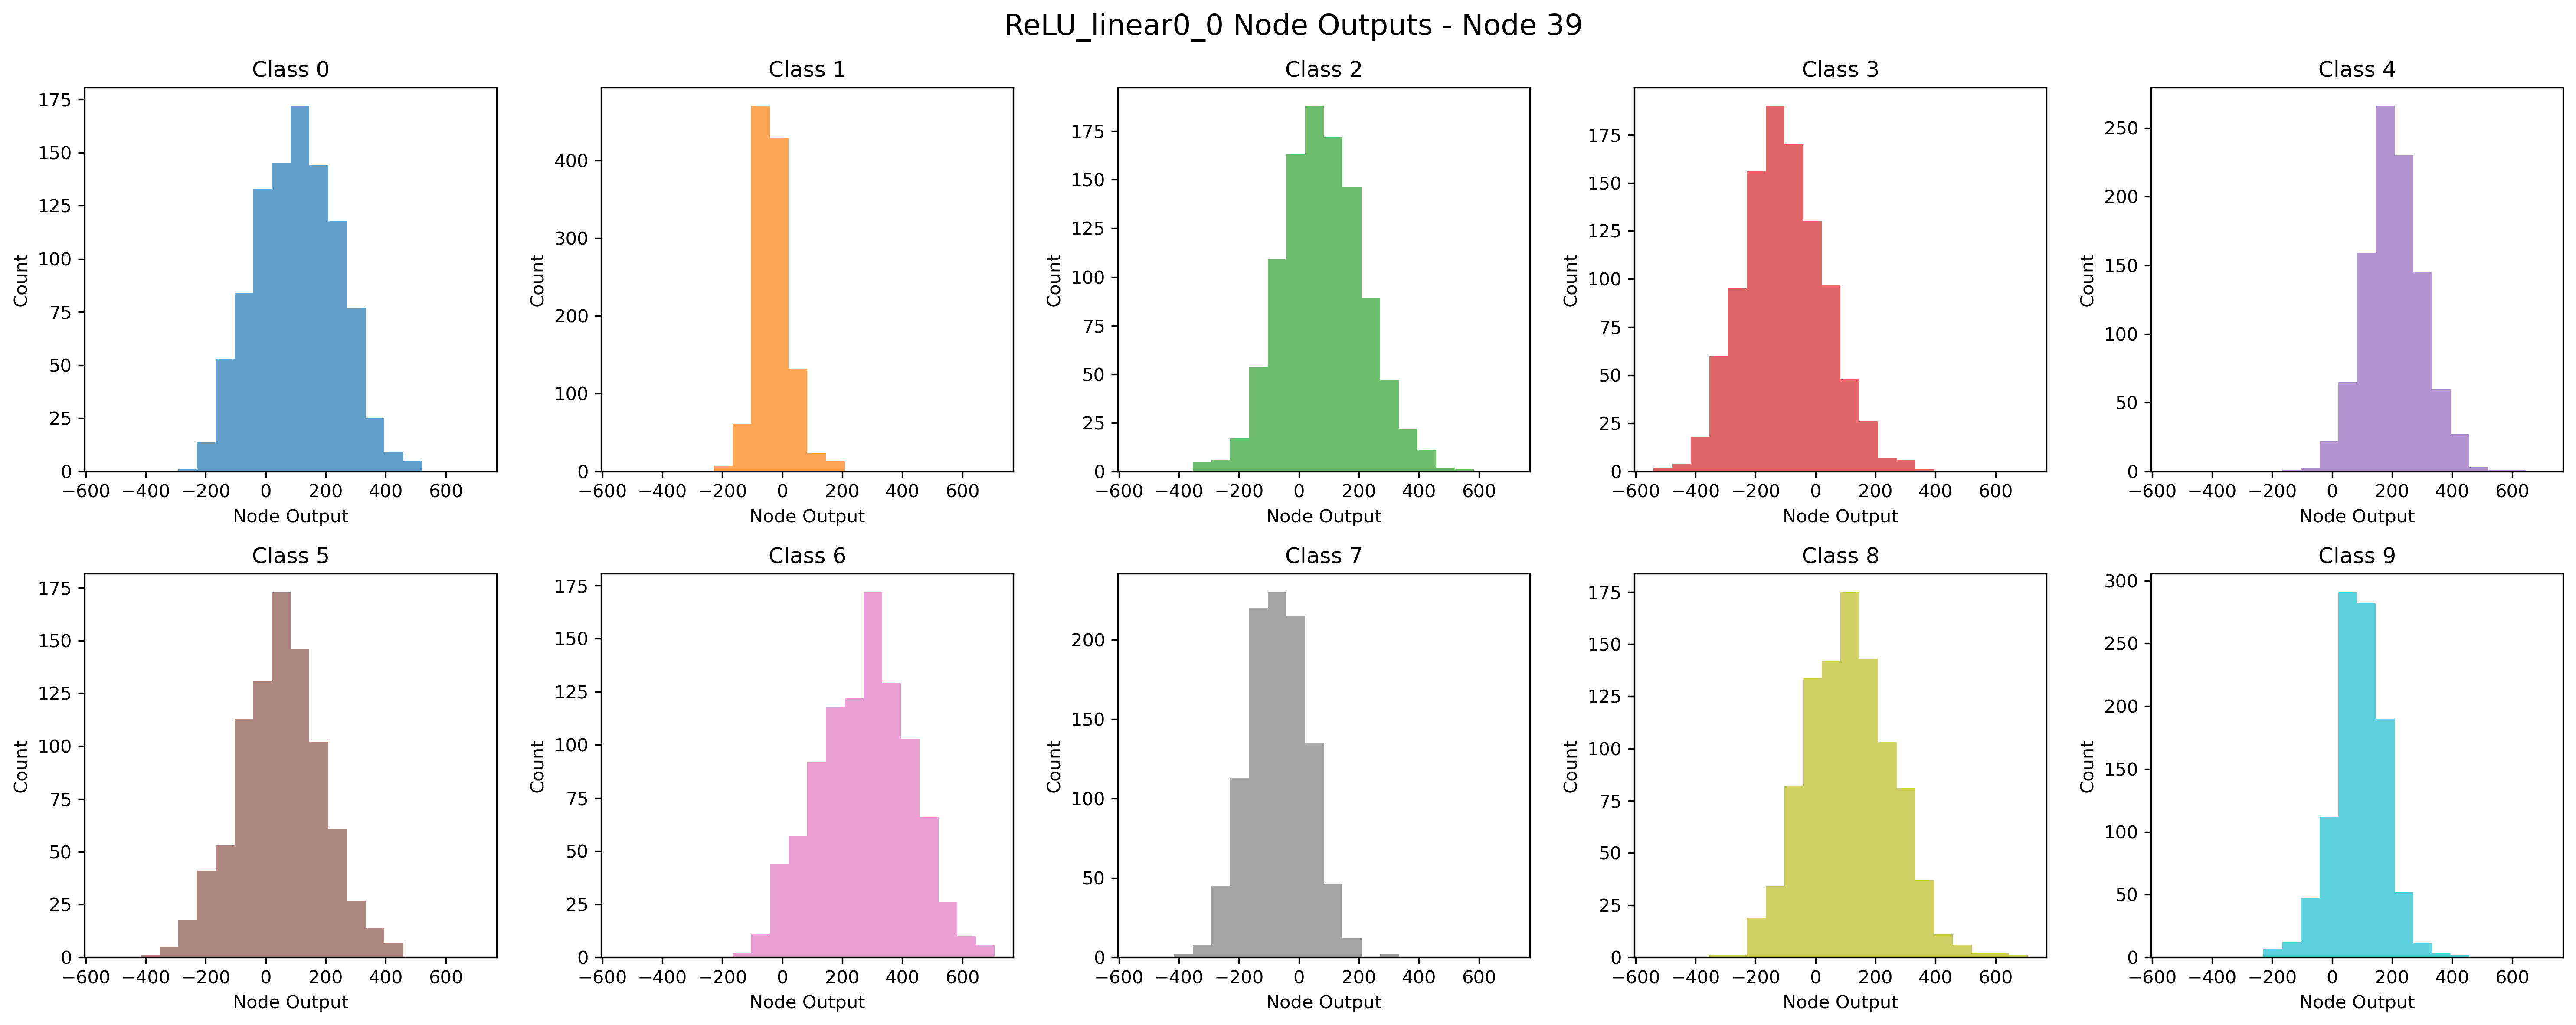
\includegraphics[width=0.8\textwidth]{images/distance_distribution}
    \caption{An example of class distributions. Each histogram reveals a cluster of points corresponding to a specific class, exhibiting heterogeneity in statistical properties such as mean, variance, skewness, and modality.}
    \label{fig:distance_distribution}
\end{figure}

Together, all of the outputs of the first linear layer form a 128-dimensional latent space. The second linear layer defines a hyperplane 
$y=Wx+b$ in 129-dimensional space, where the scalar output $y$ extends the original 128 dimensions. While most analyses of linear layers focus on linear separation, we can also interpret a hyperplane by examining the specific points it intersects within the latent space. The hyperplane defined by the second linear layer can be uniquely defined by 129 linearly independent points.

We can imagine a point $z_c$ in the 128-dimension latent space. Each element $z_c[i]$ represents the center of the class $c$ for node $i$. For each class, there is some $z_c$ that minimizes the distance to class $c$ while maximizing distance to other classes. Conversely, there is some point $z_\neg c$ that does the opposite, maximizing the distance to class $c$ while minimizing the distance to other classes. 

When the second linear layer is learning a distance representation, it is attempting to intersect 129 linearly independent points that approximate $z_c[i]$. When learning an intensity representation, it attempts to intersect 129 linearly independent points that approximate $z_\neg c$.

\subsection{Impact of Bias Exclusion}

We excluded the bias term from the second linear layer as an additional constraint to enforce the learned representation. This modification reduces the dimensionality of the solution space by one, effectively requiring the hyperplane to pass through the origin. For completeness, we conducted parallel experiments with the bias term included to assess its impact on the learned representations.

As shown in Table~\ref{tab:biased_performance}, the results are comparable to the non-biased versions. Certain models exhibit marginal improvements with the inclusion of bias, while others experience slight performance degradation. However, the general trends remain consistent across both configurations, suggesting that the bias term's influence is secondary to other architectural factors in determining overall performance.

\begin{table}[ht]
    \centering
    \begin{tabular}{lcc}
    \toprule
    \textbf{Model} & \textbf{Test Accuracy (\%)} & \textbf{Standard Deviation (\%)} \\
    \midrule
    ReLU\_Bias & $95.69$ & $0.17$ \\
    ReLU2\_Bias & $39.94$ & $18.84$ \\
    ReLU2\_Neg & $94.92$ & $0.18$ \\
    Abs\_Bias & $95.23$ & $0.16$ \\
    Abs2\_Bias & $95.38$ & $0.17$ \\
    Abs2\_Neg\_Bias & $90.53$ & $2.36$ \\
    \bottomrule
    \end{tabular}
    \caption{Performance metrics of all biased models on MNIST, including test accuracy and standard deviation.}
    \label{tab:biased_performance}
\end{table}

\subsection{Analysis of ReLU-based Architectures}

The catastrophic failure of \texttt{ReLU2} ($47.20\% \pm 12.00\%$) underscores the inherent brittleness of this architecture under intensity-based constraints. Analysis of activation patterns revealed a significant prevalence of dead nodes, with $33\%$ permanently inactive and an additional $20.5\%$ rarely active. We theorize this pattern emerges because the network is learning a disjunctive distance representation, where features that are not the target class are placed close to, or on the negative side of, the decision boundary. In the case of MNIST, this affects approximately 90\% of the samples, as each digit class represents only 10\% of the dataset.

The mechanism behind this failure can be understood in the context of the network's attempt to minimize the distances for the target class $c$ while maximizing the distances for non-target classes $\neg c$. For intensity learning to succeed, some nodes would need to place the target class at the extreme end of its activation histogram, well separated from the other classes. With a 9:1 imbalance between $\neg c$ and $c$, if the target class is not linearly separable in the 1d node spaces, the optimization process inherently pulls $c$ toward the negative side of the decision boundary along with the $\neg c$ data points. This collapse leads to widespread node inactivity, producing the observed prevalence of dead nodes.

In contrast, \texttt{ReLU2-Neg} achieved near-baseline performance ($94.93\% \pm 0.15\%$). In this architecture, the second linear layer minimizes activation for class $c$ by positioning $z_c[i]$ on the negative side of the decision boundary. Since $z_c[i]$ represents the center of class $c$'s distribution across all inputs, this positioning ensures most points from class $c$ fall on the negative side and are zeroed out after the second ReLU. This effectively suppresses activation for class $c$ while potentially maintaining positive activations for other classes to the right of the target. Although classes to the left of the target are also zeroed out, the target class still exhibits the smallest activation as long as these classes are not strongly correlated with each other. This positioning effectively minimizes the target class $c$ while maximizing $\neg c$.

\subsection{Analysis of Abs-based Architectures}

Abs networks differ from ReLU in that they cannot produce dead nodes. Instead of zeroing out negative values, Abs folds them back to the positive side, ensuring all nodes remain active. Under our distance metric theory, where zero activation indicates maximum feature membership, this architectural difference leads to distinct behaviors in how features are represented. In ReLU networks, maximum feature membership extends to all points in the negative evaluation space, creating larger feature sets. In contrast, Abs networks achieve maximum feature membership only at points exactly on the decision boundary, resulting in more focused feature sets. Since this minimum value can correspond to either $z_c$ or $z_{\neg c}$, the learned representation becomes easier to interpret.

While \texttt{Abs2} achieved strong performance ($95.35\% \pm 0.17\%$), its distance-learning counterpart \texttt{Abs2-Neg} showed significantly degraded accuracy ($90.08\% \pm 2.56\%$), with notably higher variance and a performance gap of over $5$ percentage points. Following is our theory for this performance difference.

We theorize the Abs2 hyperplane passes though $z_\neg c$, the centers of non-target classes, and Abs2-Neg hyperplane passes through $z_c$, the center of the target class. Unlike with ReLU, Abs2-Neg can actually place $z_c$ on the hyperplane and fold the values around it to larger positive values. It still learns sets of classes when there is class overlap, but the selected class sets are smaller than with ReLU.

We theorize that Abs2-Neg performs worse because there is a single optimal $z_c$. The Abs2-Neg hyperplane must pass through this optimal point and 127 additional linearly independent points to be fully defined. Since there is only one optimal $z_c$ that best separates each target class from all others, these additional points must necessarily be non-optimal separation points. These non-optimal points introduce false positives on for the target class and false negatives for the non-target classes. 

Abs2 on the other hand must select $z_{\neg c}$ for each dimension $i$. For each dimension, it can choose any of the nine non-target classes to place $z_{\neg c}[i]$, with each choice potentially creating a useful decision boundary. With nine choices for each of the 128 dimensions ($9^{128}$ possible combinations), Abs2 has an enormous space of potential solutions when selecting its hyperplane points. This combinatorial flexibility allows Abs2 to construct hyperplanes that achieve effective separation of target classes even when individual points are not optimal, as it can compensate for suboptimal choices in some dimensions by making better choices in others.

\subsection{Validation Through Additional Experiments}

Our theory about the Abs2-Neg performance drop suggests that a layer designed around a single optimal point might correct the performance difference. If our hypothesis is correct, explicitly incorporating this geometric constraint into the architecture should improve performance. We can achieve this by designing a layer that measures distance from a prototype in the latent space. Specifically, we propose a layer that computes the weighted L2 distance from a learned reference point $\mu$:

$y = \sqrt{\sum_i (\alpha_i(x_i - \mu_i))^2}$

where $\mu$ represents our hypothesized optimal point $z_c$ in the latent space, and $\alpha$ is a learnable vector of weights that allows the network to selectively focus on different dimensions of the input space. This formulation directly embeds our geometric intuition: the layer explicitly learns a single reference point and measures distance from it, rather than implicitly discovering such points through hyperplane positioning as in Abs2-Neg.

We refer to this architecture as OffsetL2. While Abs2-Neg must construct its hyperplane through $z_c$ and 127 additional points that may not be optimal for class separation, OffsetL2 directly optimizes a single prototype $\mu$ and its associated importance weights $\alpha$. This design eliminates the need for the network to discover implicit geometric relationships through hyperplane positioning, instead allowing it to learn an explicit optimal reference point for each class. The $\alpha$ weights provide flexibility similar to Abs2's ability to emphasize different input dimensions, but do so through direct scaling rather than through the indirect mechanism of hyperplane orientation.

We expect this architecture to perform well for both distance and intensity learning, since it can learn either the optimal $z_c$ or $z_{\neg c}$ as its prototype. The flexibility provided by $\alpha$ allows the network to appropriately weight the dimensions of the latent space regardless of which reference point is being learned.
When we incorporate OffsetL2 into the Abs2-Neg model and combine it with the LogSoftmax function used in CrossEntropyLoss, the resulting architecture bears a striking resemblance to Radial Basis Function (RBF) networks. The key equations highlight this similarity:
OffsetL2 + LogSoftmax:

$y = -\log(\exp(\sqrt{\sum_i (\alpha_i(x_i - \mu_i))^2}))$

Traditional RBF:

$y = -\log(\exp(\sqrt{\sum_i (x_i - \mu_i)^2}))$

The primary distinction lies in our inclusion of the learnable weight vector $\alpha$, which allows the network to modulate the importance of different dimensions in computing the distance from the prototype. This connection to RBF networks provides an interesting theoretical foundation for understanding our architecture's strong performance.

Initial experiments suggested that the OffsetL2 models had not fully converged after our standard training protocol of 5000 epochs. To establish performance limits and ensure fair comparison, we extended the training duration to 50000 epochs for both the new OffsetL2 architectures and our original baseline models. The extended training of all ten models was completed in approximately 8 hours on an NVIDIA RTX 3070 Ti GPU.

\begin{table}[ht]
    \centering
    \begin{tabular}{lcccc}
    \toprule
    \textbf{Model} & \textbf{Accuracy (\%)} & \textbf{Std Dev (\%)} & \textbf{Min (\%)} & \textbf{Max (\%)} \\
    \midrule
    % Baseline Models
    ReLU\_Bias & 96.62 & 0.17 & 96.19 & 96.88 \\
    ReLU2\_Bias & 56.31 & 19.31 & 28.60 & 96.24 \\
    ReLU2\_Neg & 96.46 & 0.17 & 96.21 & 96.79 \\
    Abs\_Bias & 95.87 & 0.22 & 95.45 & 96.24 \\
    Abs2\_Bias & 95.95 & 0.17 & 95.56 & 96.25 \\
    Abs2\_Neg\_Bias & 92.25 & 2.07 & 87.61 & 95.39 \\
    \midrule
    % OffsetL2 Models
    ReLU-L2 & 97.33 & 0.13 & 97.13 & 97.57 \\
    ReLU-L2-Neg & 97.36 & 0.14 & 97.11 & 97.72 \\
    Abs-L2 & 97.61 & 0.07 & 97.47 & 97.77 \\
    Abs-L2-Neg & 97.56 & 0.09 & 97.43 & 97.73 \\
    \bottomrule
    \end{tabular}
    \caption{Performance metrics across all models with extended training (50000 epochs), averaged over 20 runs.}
    \label{tab:extended_training}
\end{table}

The extended training results, summarized in Table~\ref{tab:extended_training}, reveal several significant findings. The baseline models showed modest improvements, with ReLU2\_Neg achieving 96.46\% $\pm$ 0.17\% accuracy and ReLU\_Bias reaching 96.62\% $\pm$ 0.17\%. However, ReLU2\_Bias continued to exhibit unstable performance (56.31\% $\pm$ 19.31\%), and Abs2\_Neg\_Bias maintained its performance gap (92.25\% $\pm$ 2.07\%).

The OffsetL2 architectures demonstrated substantial improvements over their baseline counterparts. Most strikingly, both Abs-L2 and Abs-L2-Neg achieved nearly identical performance (97.61\% $\pm$ 0.07\% and 97.56\% $\pm$ 0.09\% respectively), effectively eliminating the performance gap observed in their baseline versions. This convergence strongly supports our geometric theory about the importance of explicit prototype learning.

The ReLU variants of OffsetL2 also showed remarkable improvement and stability, with ReLU-L2 and ReLU-L2-Neg achieving 97.33\% $\pm$ 0.13\% and 97.36\% $\pm$ 0.14\% respectively. Notably, ReLU-L2 completely avoided the catastrophic failure modes observed in ReLU2\_Bias, suggesting that the explicit prototype learning provides a more stable optimization landscape.

The consistently lower standard deviations in the OffsetL2 models (all $\leq$ 0.14\%) compared to their baseline counterparts indicates that explicit prototype learning not only improves performance but also leads to more reliable training outcomes. This stability, combined with the superior accuracy across all OffsetL2 variants, validates our hypothesis that explicitly modeling the geometric constraints of the learning problem leads to better solutions.

The superior performance of the OffsetL2 architecture can be directly traced to its mathematical foundations. While previous architectures approximated individual components of the Mahalanobis distance calculation, OffsetL2 explicitly implements the original Mahalanobis distance equation by computing the L2 norm of whitened distances from learned prototypes. This direct implementation of the underlying statistical theory - moving from approximation to explicit calculation - manifests in both improved accuracy ($\geq97.5\%$) and notably reduced variance across all variants. The consistency between the mathematical framework and empirical results provides strong validation of the theoretical connection between neural networks and Mahalanobis distance.

\subsection{Conclusion}

Our analysis reveals fundamental insights into how neural networks learn and represent features through the lens of statistical distances. The catastrophic failure of ReLU2 exposed how intensity-based constraints can create untenable optimization landscapes when the majority of inputs must be positioned on the negative side of decision boundaries. Meanwhile, the underperformance of Abs2-Neg compared to Abs2 illuminates the geometric constraints at play: while Abs2 can leverage multiple optimal separation points across its high-dimensional space, Abs2-Neg must work with a more restricted set of optimal points, leading to increased false positives and degraded performance. These findings suggest that the success or failure of different activation functions may have less to do with their intrinsic properties and more to do with how they interact with the geometric constraints of the feature space. Understanding these geometric interactions and constraints provides valuable guidance for future neural network designs, as demonstrated by our supplementary experiments with OffsetL2 architectures, where explicit incorporation of these geometric principles led to enhanced performance across all variants. Together, these results demonstrate the value of analyzing neural networks through the framework of statistical distance measures, offering new perspectives on both their capabilities and limitations that can inform more principled architectural decisions.